% 第3章
\chapter{パラメータに関する考察}
\section{実験目的}
本章では,二足歩行ロボットの歩行パターン生成のパラメータによって波形にどのような影響を与えているかを検証する.
検証するパラメータはControl Horizon,Q / R,start with this stepである.また,各パラメータごとに実行時間を記録する.

\section{実験結果}

\subsection{Control Horizon}
\begin{figure}[H]
  \centering
 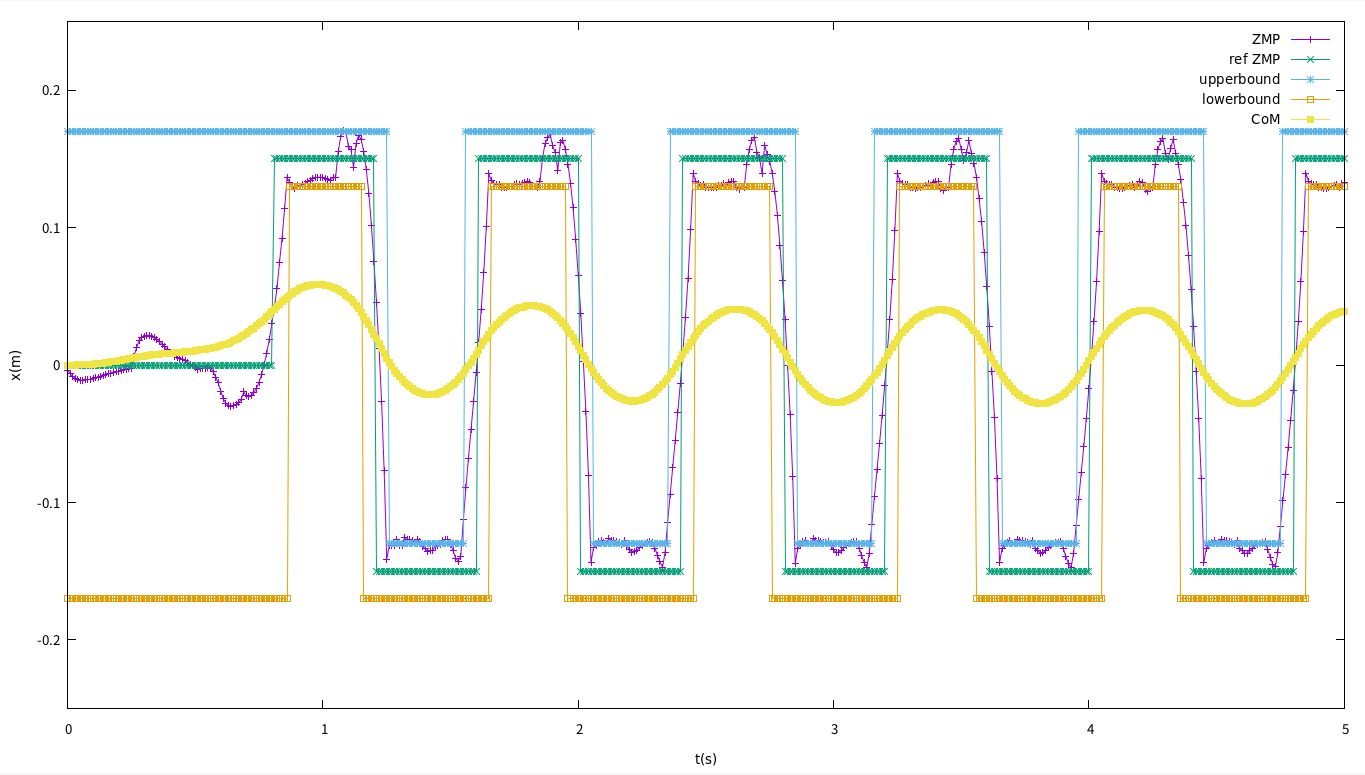
\includegraphics[keepaspectratio, scale=0.25]
      {images/mpc_horizon/mpc_horizon_100.png}
 \caption{Illustration of table-cart model}
 \label{Fig:Illustration of table-cart model}
\end{figure}

\begin{figure}[H]
  \centering
 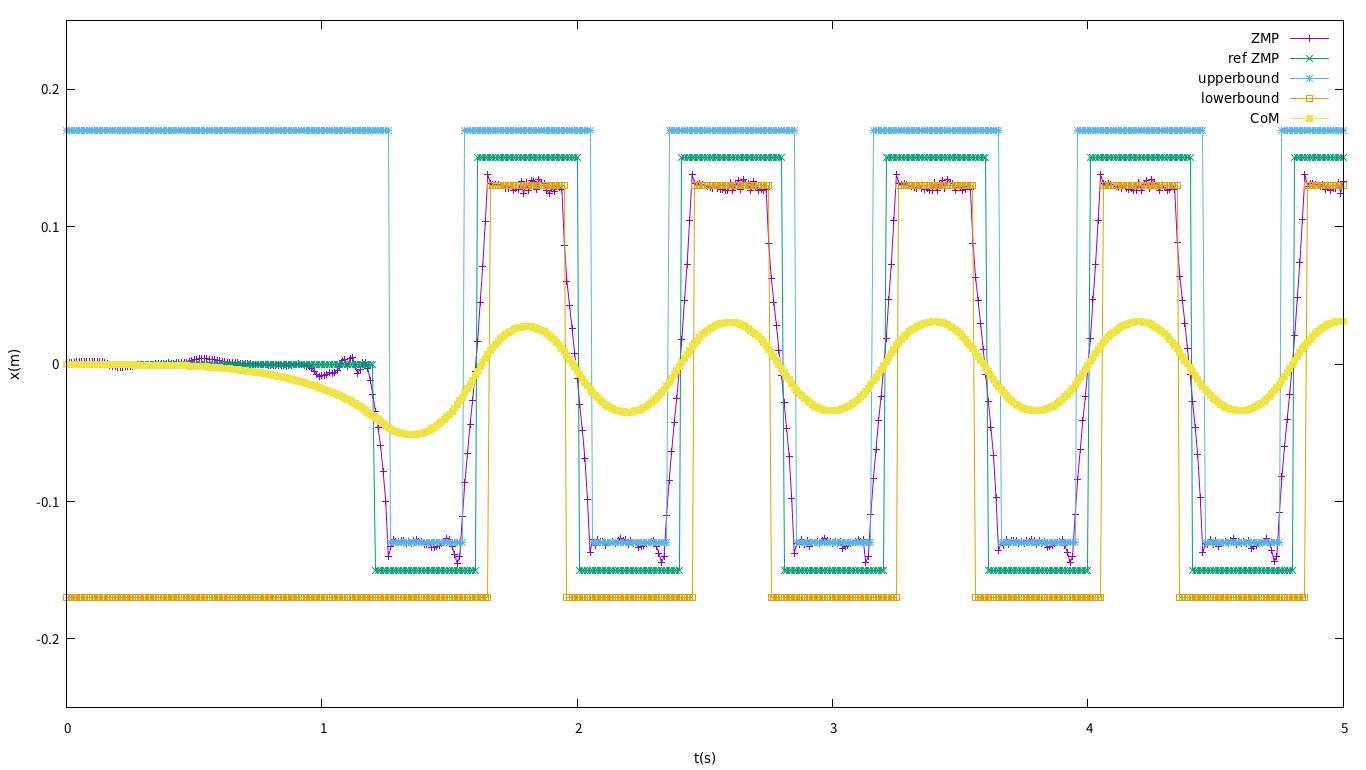
\includegraphics[keepaspectratio, scale=0.25]
      {images/mpc_horizon/mpc_horizon_150.png}
 \caption{Illustration of table-cart model}
 \label{Fig:Illustration of table-cart model}
\end{figure}

\begin{figure}[H]
  \centering
 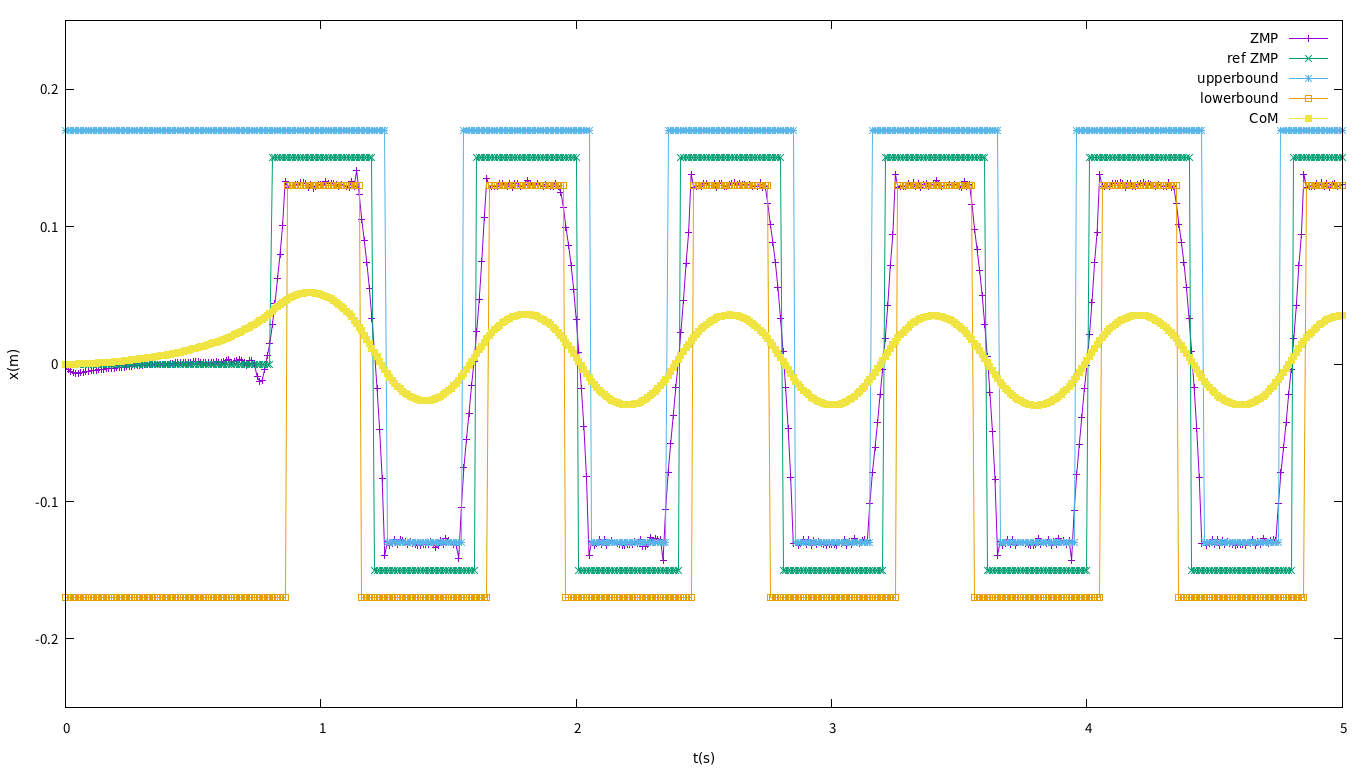
\includegraphics[keepaspectratio, scale=0.25]
      {images/mpc_horizon/mpc_horizon_200.png}
 \caption{Illustration of table-cart model}
 \label{Fig:Illustration of table-cart model}
\end{figure}

\begin{figure}[H]
  \centering
 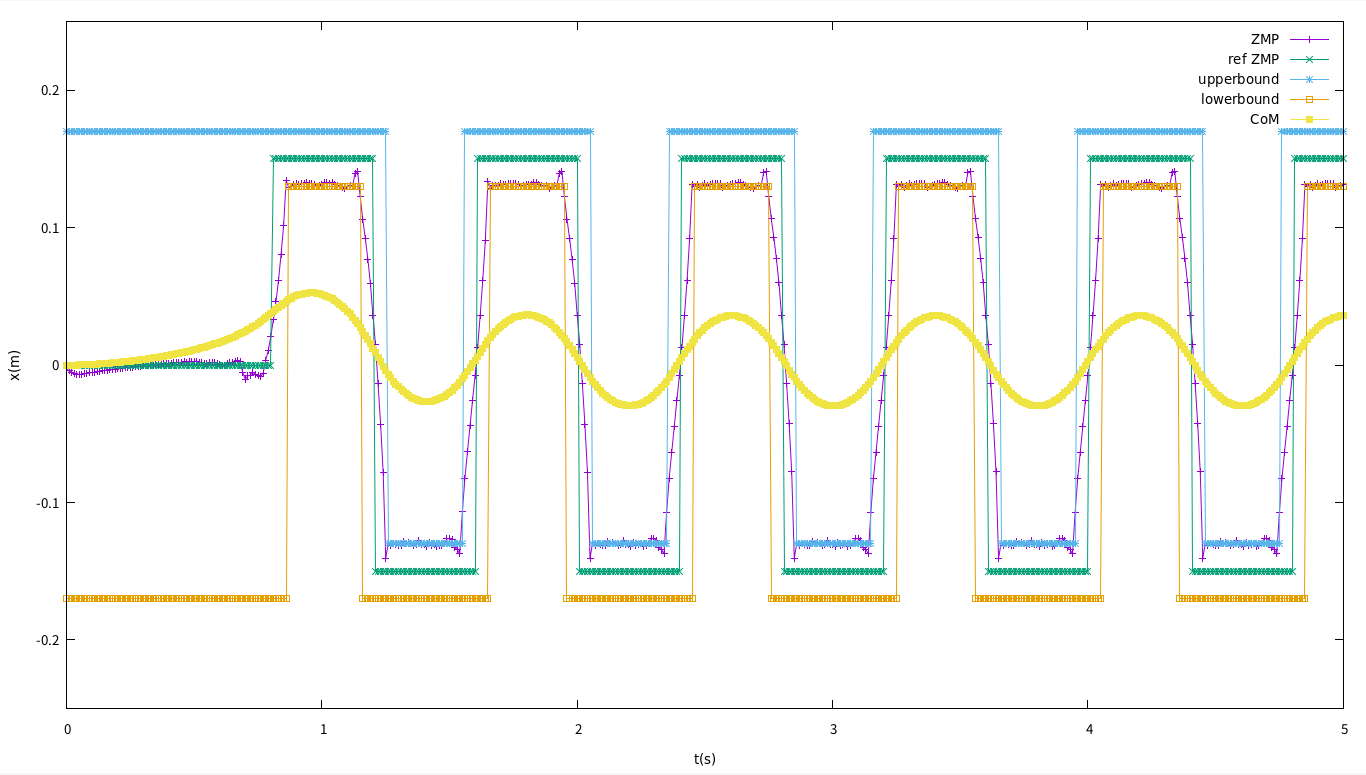
\includegraphics[keepaspectratio, scale=0.25]
      {images/mpc_horizon/mpc_horizon_250.png}
 \caption{Illustration of table-cart model}
 \label{Fig:Illustration of table-cart model}
\end{figure}

\begin{figure}[H]
  \centering
 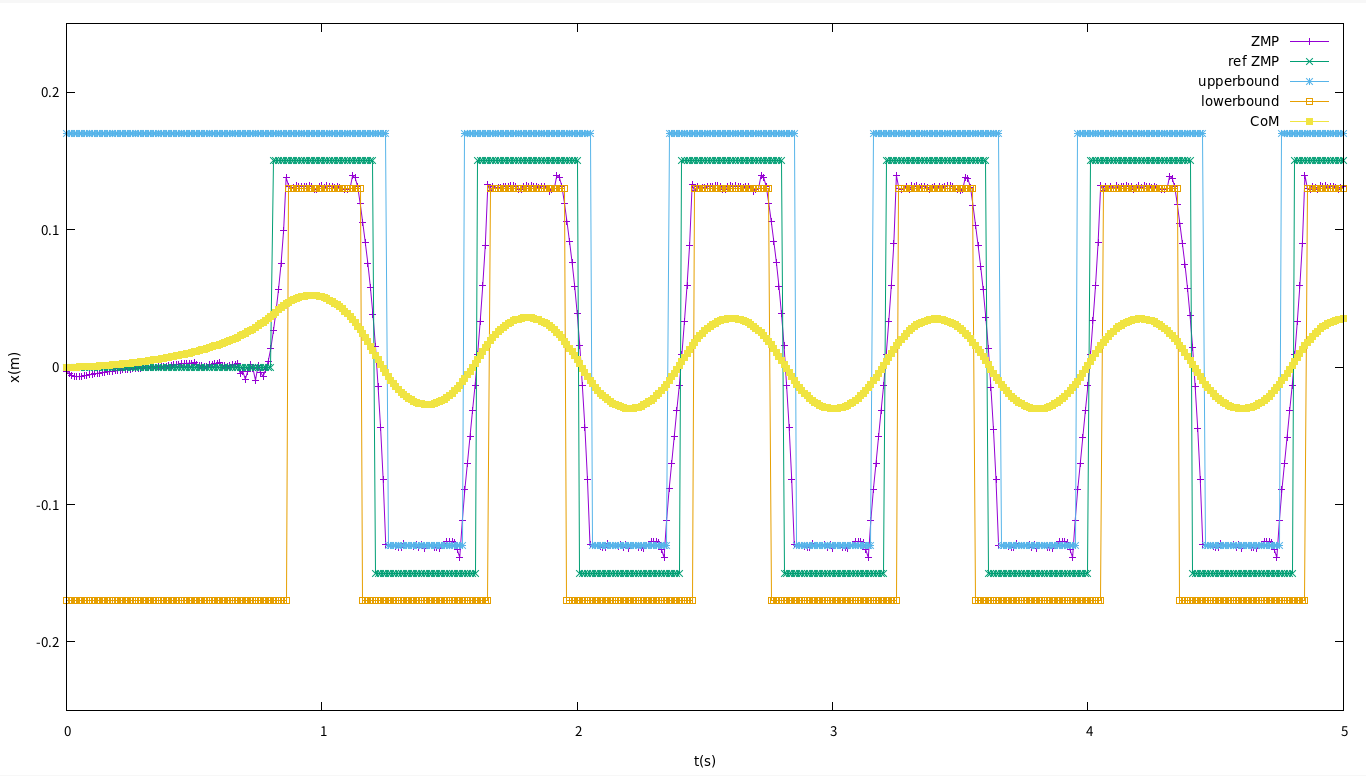
\includegraphics[keepaspectratio, scale=0.25]
      {images/mpc_horizon/mpc_horizon_300.png}
 \caption{Illustration of table-cart model}
 \label{Fig:Illustration of table-cart model}
\end{figure}

%---------------------------------------------------------
\subsection{Q / R}
\begin{figure}[H]
  \centering
 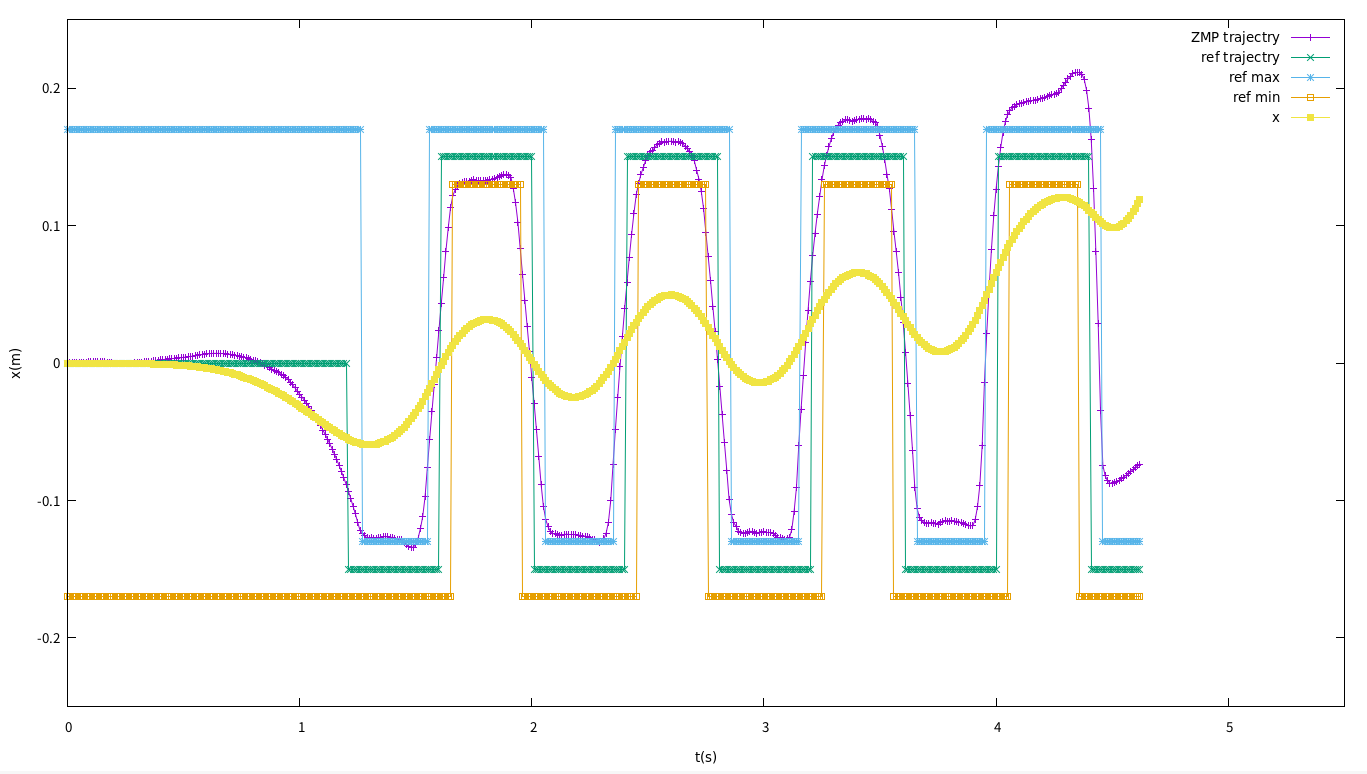
\includegraphics[keepaspectratio, scale=0.25]
      {images/mpc_qr/mpc_qr_10_4_error.png}
 \caption{Illustration of table-cart model}
 \label{Fig:Illustration of table-cart model}
\end{figure}

\begin{figure}[H]
  \centering
 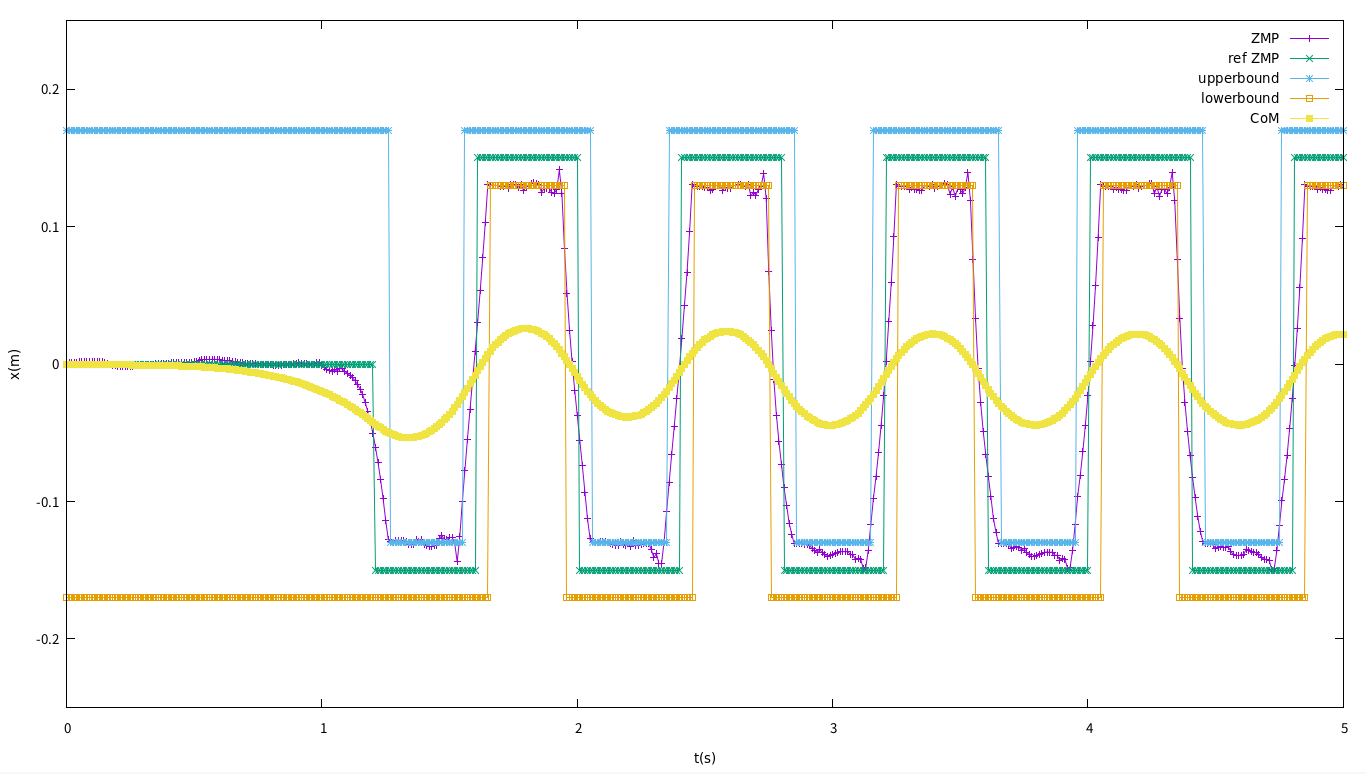
\includegraphics[keepaspectratio, scale=0.25]
      {images/mpc_qr/mpc_qr_10_5.png}
 \caption{Illustration of table-cart model}
 \label{Fig:Illustration of table-cart model}
\end{figure}

\begin{figure}[H]
  \centering
 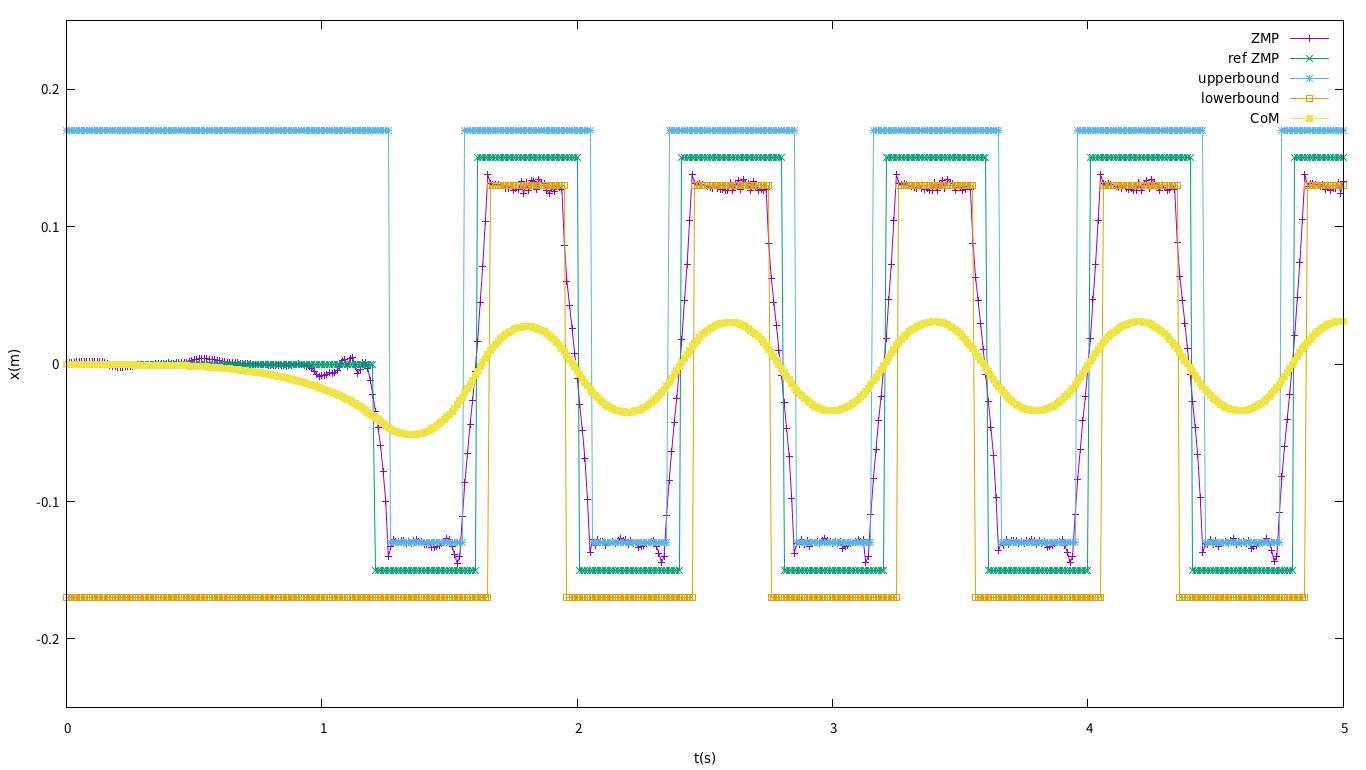
\includegraphics[keepaspectratio, scale=0.25]
      {images/mpc_qr/mpc_qr_10_6.png}
 \caption{Illustration of table-cart model}
 \label{Fig:Illustration of table-cart model}
\end{figure}

\begin{figure}[H]
  \centering
 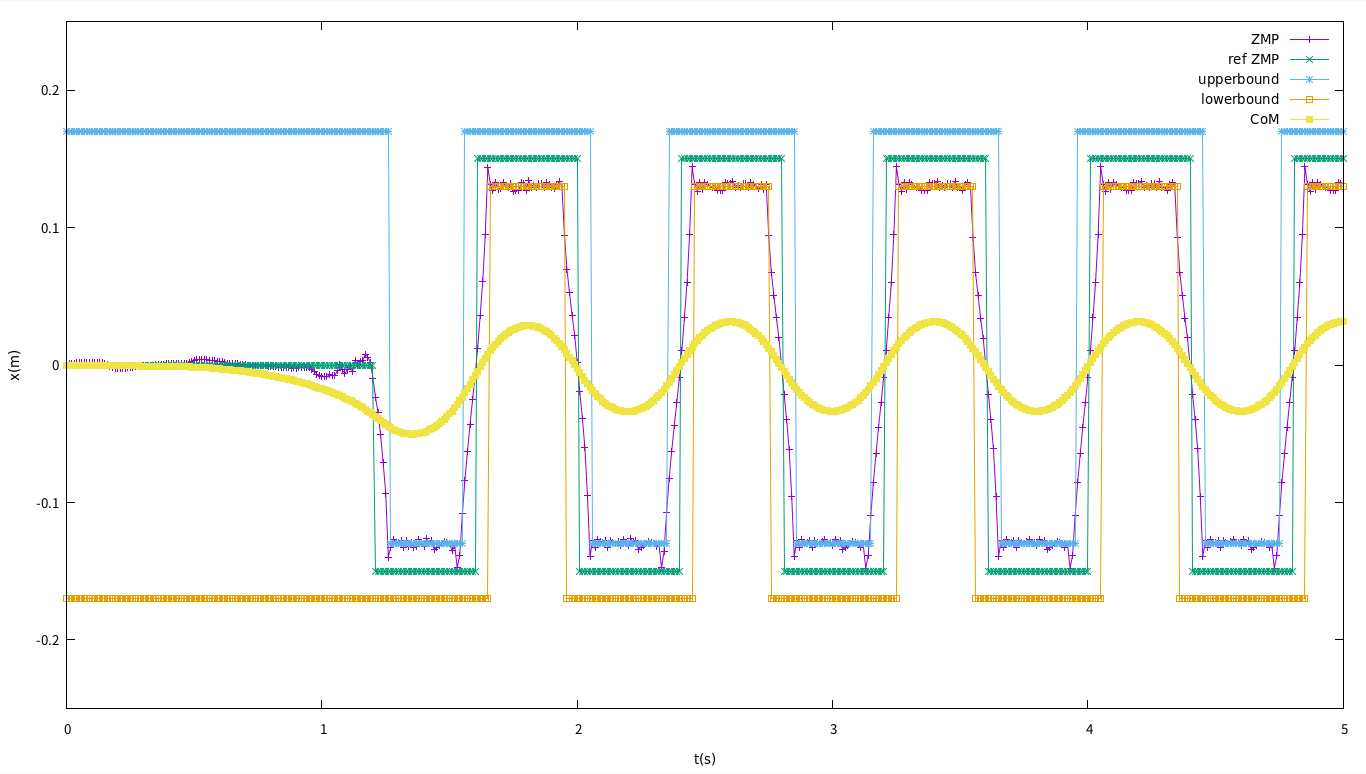
\includegraphics[keepaspectratio, scale=0.25]
      {images/mpc_qr/mpc_qr_10_7.png}
 \caption{Illustration of table-cart model}
 \label{Fig:Illustration of table-cart model}
\end{figure}

\begin{figure}[H]
  \centering
 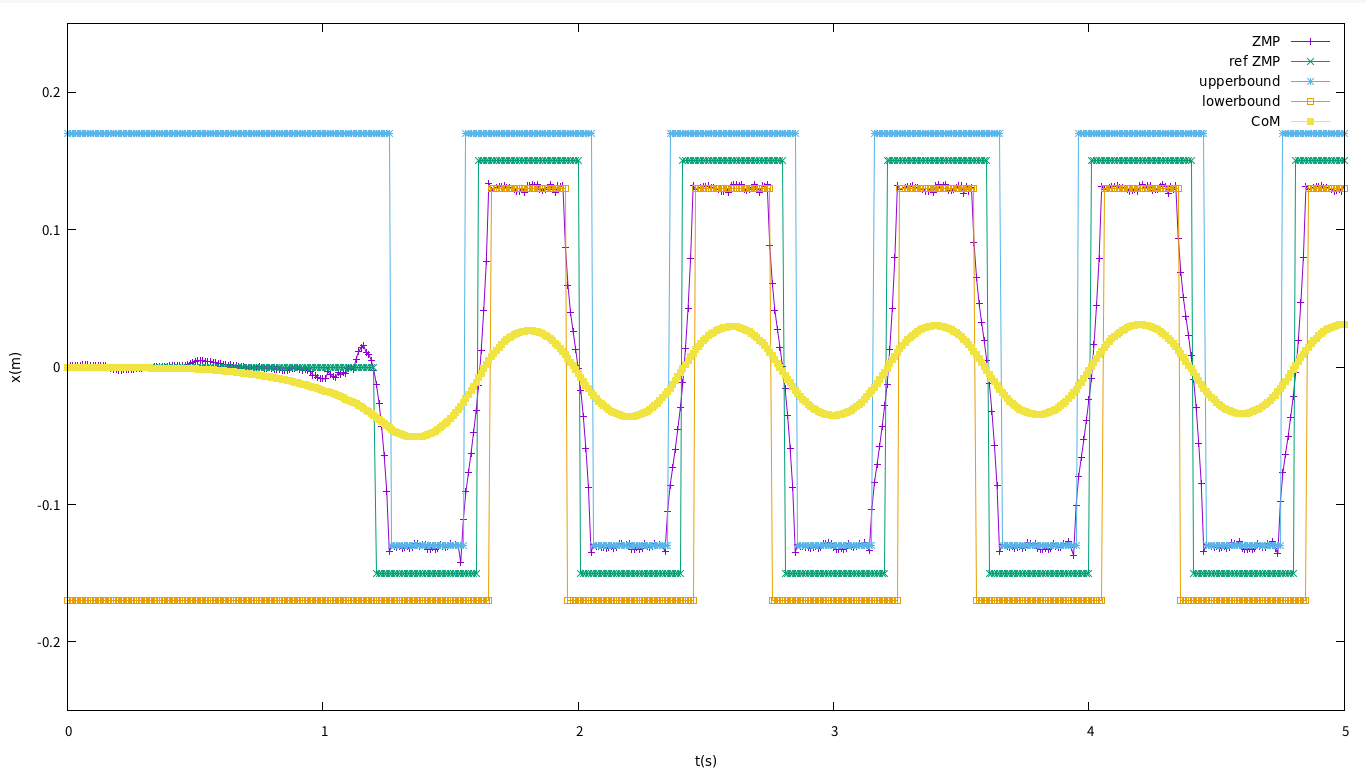
\includegraphics[keepaspectratio, scale=0.25]
      {images/mpc_qr/mpc_qr_10_8.png}
 \caption{Illustration of table-cart model}
 \label{Fig:Illustration of table-cart model}
\end{figure}

\begin{figure}[H]
  \centering
 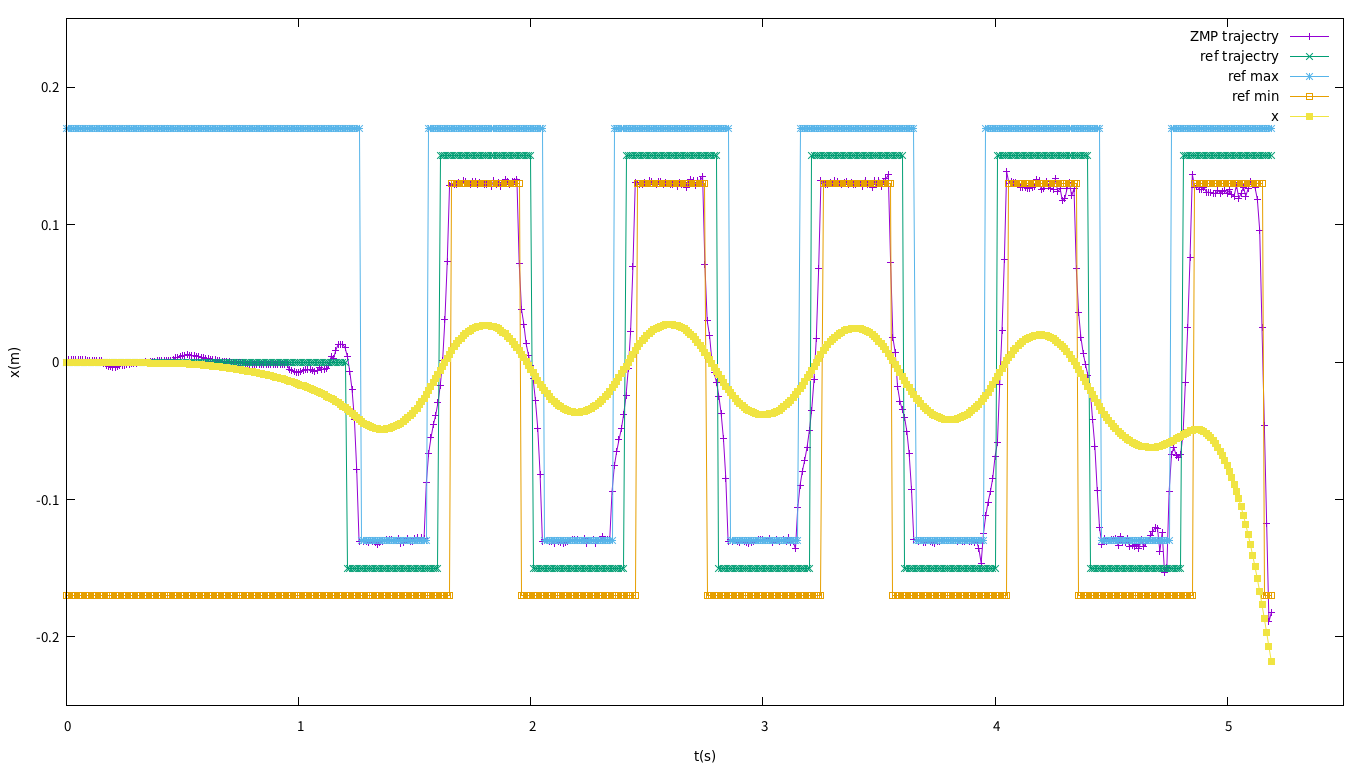
\includegraphics[keepaspectratio, scale=0.25]
      {images/mpc_qr/mpc_qr_10_9_error.png}
 \caption{Illustration of table-cart model}
 \label{Fig:Illustration of table-cart model}
\end{figure}

%-----------------------------------------------------------------
\subsection{start with this step}


\begin{figure}[H]
  \centering
 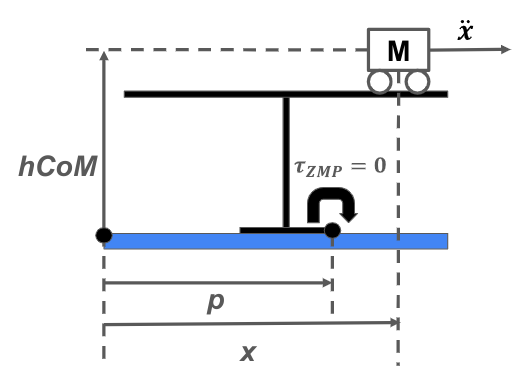
\includegraphics[keepaspectratio, scale=0.5]
      {images/walk/table.png}
 \caption{Illustration of table-cart model}
 \label{Fig:Illustration of table-cart model}
\end{figure}

\newpage
%--------------------------------------------------------
\section{実行時間}
 この節では,4.2で出力したソフトウェアの実行時間を計測する.
計測は各パラメータをそれぞれ10回ずつ行い,平均時間を記録する.表に示す.「x」は生成できていないため対象外とする.
\begin{table}[hbtp]
  \centering
  \caption{Execution time of each Q/R}
  \label{Execution time of each Q/R}
  \begin{tabular}{|l|l|l|l|l|l|l|}
  \hline \hline
  Q / R        & 10\textasciicircum{}4 & 10\textasciicircum{}5 & 10\textasciicircum{}6 & 10\textasciicircum{}7 & 10\textasciicircum{}8 & 10\textasciicircum{}9 \\ \hline
  time {[}s{]} & x                     & 4.2                   & 5.6                   & 5.6                   & 5.1                   & x                     \\ \hline
  \end{tabular}
\end{table}

\begin{table}[hbtp]
  \centering
  \caption{Execution time of each Control Horizon}
  \label{Execution time of each Control}
  \begin{tabular}{|l|l|l|l|l|l|l|}
  \hline \hline
  Control Horizon {[}s{]} & 0.5 & 1.0 & 1.5 & 2.0 & 2.5  & 3.0  \\ \hline
  time {[}s{]}            & x   & 3.7 & 5.6 & 9.5 & 12.2 & 15.0 \\ \hline
  \end{tabular}
\end{table}

%---------------------------------------------------------------------
\section{パラメータの傾向}

 Control Horizon
Q/R
実行時間
%Q/Rの値は$10\textasciicircum{}5$と$10\textasciicircum{}5$の間は1秒の差があるが,その他の値は上げても実行時間に大きな差はなかった.
Control Horizonは最適化問題を解く区間が長くなったため実行時間は比例した.
\newpage